%------------------------------------------------
\chapter{Projeto dos Módulos}\label{ProjetoDosModulos}
%---------------------------------------------------------

\section{Introdução}
O projeto de uma solução para atendimento dos requisitos propostos neste trabalho exige atenção principalmente ao consumo de energia, dada a baixa disponibilidade desta por longos intervalos de tempo. É necessário que sejam projetados sistemas que executem suas funções de forma eficaz, rápida e com o mínimo consumo.

Na Figura \ref{fig:diagram} é apresentado o diagrama de blocos proposto. Nele são observados 8 módulos internos ao \textit{chip} e um módulo externo, denominado \emph{Ajuste Externo}. Esta solução é proposta com base nos trabalhos apresentados por \citeonline{YEAGER:2009}, \citeonline{YEAGER:2010} e \citeonline{YEAGER:2010:2}. O módulo \emph{Circuito de Casamento} apresentado não é tratado neste trabalho, uma vez que não é primordial para o circuito de alimentação da etiqueta.

\begin{figure}[!htb]
	\caption[Diagrama de blocos do sistema proposto]{\label{fig:diagram}Diagrama de blocos do sistema proposto}
	\begin{center}
		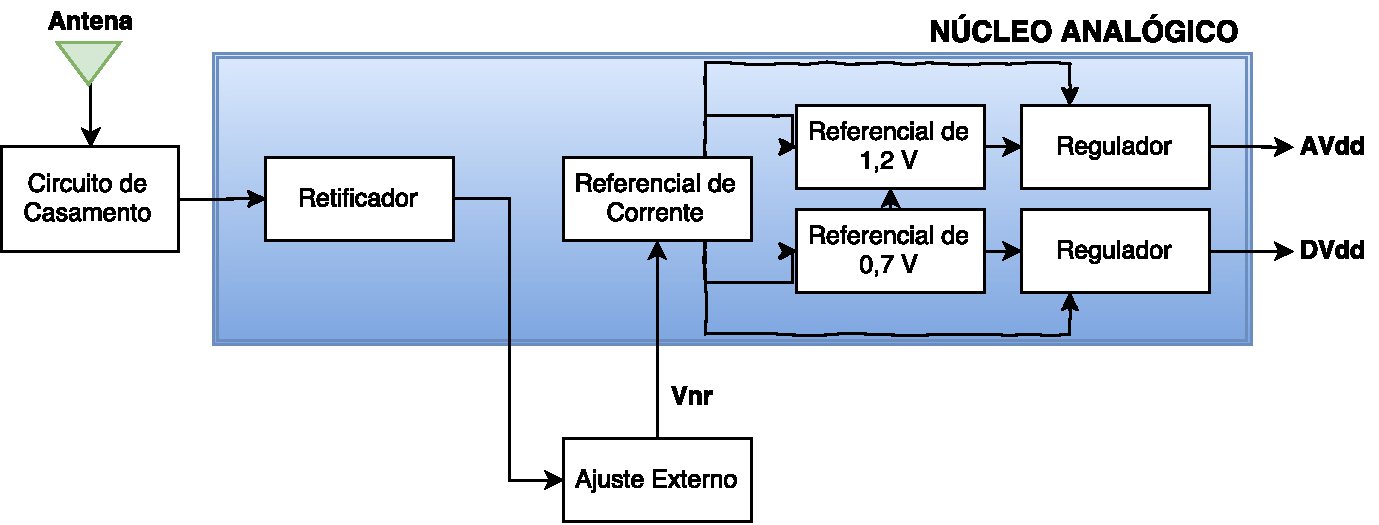
\includegraphics[width=1\linewidth]{diagram.pdf}
	\end{center}
	\legend{A região na área azul corresponde aos componentes em \textit{chip} propostos para o núcleo analógico. Fonte: adaptado de \citeonline{YEAGER:2009}}
\end{figure}

Na Figura \ref{fig:schematic} é exibido um esquemático mais detalhado do núcleo analógico e o relacionamento interno entre os componentes. A \emph{Região 1} diz respeito à antena e um circuito para ajuste de máxima transferência de potência, tema discutido por \citeonline{VITA:2005}, que pode, ou não, já estar presente na antena. Dela o sinal é transmitido ao retificador, que eleva o nível de tensão do sinal de entrada, gerando o sinal $V_{ret}$.

\begin{figure}[!htb]
	\caption{\label{fig:schematic}Esquemático do circuito com todos os módulos propostos}
	\begin{center}
		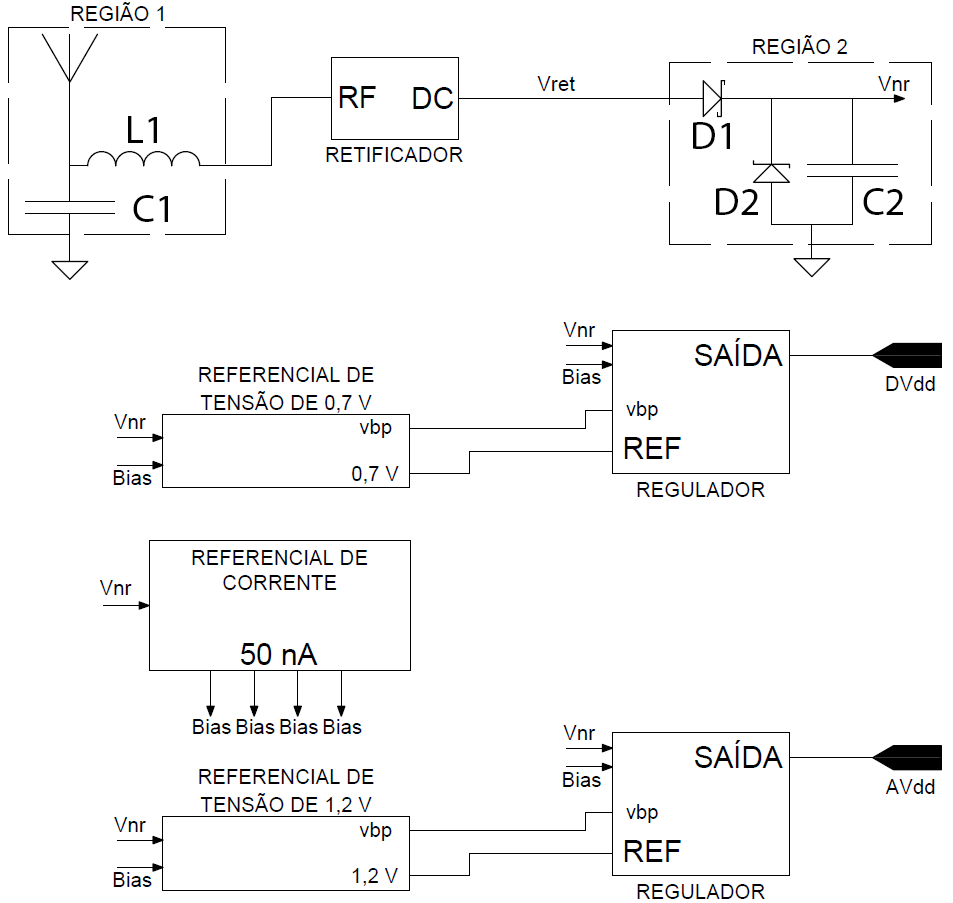
\includegraphics[width=0.95\linewidth]{schematic.png}
	\end{center}
	\legend{Fonte: adaptação de \citeonline{YEAGER:2009}}
\end{figure}

A \emph{Região 2} é o bloco chamado de \emph{Ajuste Externo} na Figura \ref{fig:diagram}. Constituída por um diodo \textit{schottky} ({D1}), um diodo zener ({D2}) e um capacitor de valor elevado (\citeonline{YEAGER:2009} utilizou 10 $\mu$F), sua função é prover a fonte de tensão não-regulada, $V_{nr}$, que alimentará os demais módulos do sistema. Essa tensão é gerada a partir do ceifamento de $V_{ret}$ e da carga do capacitor, que agirá como fonte da tensão não-regulada. {D1}, neste módulo, opera como uma resistência para controle da carga do capacitor {C2}. Já {D2} serve dois propósitos: o primeiro de garantir o limite superior de $V_{nr}$; e o segundo de servir como escoamento para o excedente de potência absorvido pelo retificador.

A justificativa para o uso de um capacitor com valor elevado é a de que ele agirá como fonte para o restante do circuito. Segundo \citeonline{YEAGER:2009}, os leitores comerciais costumam trabalhar com ciclo de trabalho inferior a 50\%, tornando necessária a existência de um dispositivo armazenador de energia. Caso um leitor com ciclo de trabalho unitário fosse utilizado, capacitores menores poderiam ser utilizados. Outra justificativa para o uso de um capacitor tão elevado é a de que ele também funcionaria como fonte de energia para o microcontrolador utilizado na aplicação. Neste trabalho não há abordagem específica acerca do núcleo analógico.

Todos os módulos apresentados na Figura \ref{fig:schematic} são alimentados pela tensão não-regulada. Correntes referência de $50~nA$ são utilizadas para polarizar os transistores operando como dreno de corrente nos referenciais de tensão e reguladores. Essas correntes são oriundas de um referencial de corrente do tipo $\dfrac{V_{GS}}{R}$. Os referenciais de tensão são obtidos a partir de circuitos do tipo \textit{bandgap}, um para $1,2~V$ e outro para $0,7~V$. Os reguladores foram modelados como amplificadores com ganho unitário (operando como \textit{buffers}), drenando corrente de $V_{nr}$.

A metodologia utilizada consistiu em projetar os módulos individualmente e avaliá-los sob diferentes situações para, então, analisar o comportamento do sistema como um todo. As seções a seguir tratam da análise envolvida no projeto, desenvolvimento e testes de cada um.


\section{Retificador}
O retificador é um elemento crucial no desenvolvimento de um \textit{front-end} analógico. Seu rendimento é um fator primordial para o funcionamento regular do sistema. Uma falha na modelagem deste módulo repercute em todos os demais.

Diversos trabalhos tratam da modelagem de retificadores e do estudo do seu impacto em etiquetas passivas. \citeonline{KARTHAUS:2003}, \citeonline{UMEDA:2006}, \citeonline{KOCER:2004}, \citeonline{VITA:2005}, \citeonline{YI:2007}, \citeonline{LE:2008} e \citeonline{BARNETT:2006} utilizam uma topologia NMOS tradicional, adotada por \citeonline{YEAGER:2009} e utilizada neste estudo. \citeonline{BARNETT:2006}, especialmente, analisam as impedâncias de entrada e saída de dobradores de tensão e retificadores multiníveis, com ênfase na relação entre as dimensões dos transistores e na quantidade de estágios e como estas variáveis afetam as impedâncias e o custo do sistema. \citeonline{MANDAL:2007} propõem uma topologia CMOS e fundamentam a teoria com embasamentos matemático e de simulação. \citeonline{NAKAMOTO:2006} apresentam resultados observados com topologias NMOS e CMOS distintas das anteriormente citadas.

Na Tabela \ref{tab:ret_comp} são expostos resultados comparativos entre diversas aplicações da mesma topologia utilizada neste trabalho. Os resultados alcançados por \citeonline{NAKAMOTO:2006} e \citeonline{LE:2008} possuem um ponto em comum: suas otimizações da topologia convencional buscam ajustar o valor da tensão limiar $V_t$ dos transistores de modo a melhorar a eficiência e sensibilidade do retificador. Eles alcançam os melhores resultados até o momento: $1~V$ de saída é reportado com $-22,5~dBm$ de potência de entrada. \cite{YEAGER:2009}.

\begin{table}[!htb]
	\centering
	\caption{\label{tab:ret_comp}Comparação da performance de retificadores}
	\begin{tabular}{c|ccccc}
		\multirow{2}{*}{\textbf{Autor}} & \textbf{Le} & \textbf{Umeda} & \textbf{Nakamoto} & \textbf{Karthaus} & \textbf{Kocer} \\ & \textbf{(2008)} & \textbf{(2006)} & \textbf{(2006)} & \textbf{(2003)} & \textbf{(2004)} \\
		\hline
		\textbf{Tecnologia} & 0,25 $\mu$m & 0,30 $\mu$m & 0,35 $\mu$m & 0,50 $\mu$m & 0,25 $\mu$m \\
		\hline
		\textbf{Máximo Rendimento} & 60\% & 33\% & 24\% & 28\% & 11\% \\
		\hline
		\textbf{Potência RF Mínima} & 5,5 $\mu$W & 40 $\mu$W & 100 $\mu$W & 16,7 $\mu$W & 60 $\mu$W \\
		\hline
		\multirow{2}{*}{} \textbf{Distância Máxima} & 42 m & 17 m & 11 m & 26 m & 13 m \\ \textbf{Teórica} & @ 4 W & @ 4 W & @ 4 W & @ 4 W & @ 4 W \\
		\hline
		\multirow{2}{*}{} \textbf{Distância Máxima} & 15 m & 2 m & 4,3 m & 4,5 m & 1,7 m \\ \textbf{Medida} & @ 4 W & @ 4 W & @ 4 W & @ 1 W & @ 60 mW \\
	\end{tabular}
	\legend{Fonte: \citeonline{LE:2008}}
\end{table}

A característica mais crucial no projeto de um retificador é a tensão limiar $V_t$ dos componentes utilizados \cite{YEAGER:2009}. A tecnologia utilizada possui transistores de $V_t$ padrão, baixo e nulo. Levando-se em consideração os estudos supracitados, utilizou-se transistores de $V_t$ nulo. O dimensionamento foi feito segundo os critérios de \citeonline{YEAGER:2009}, com o intuito de otimizar a impedância de entrada do sistema.

\begin{figure}[!h]
	\caption{\label{fig:rectifier_cell}Esquemático da célula utilizada no retificador}
	\begin{center}
		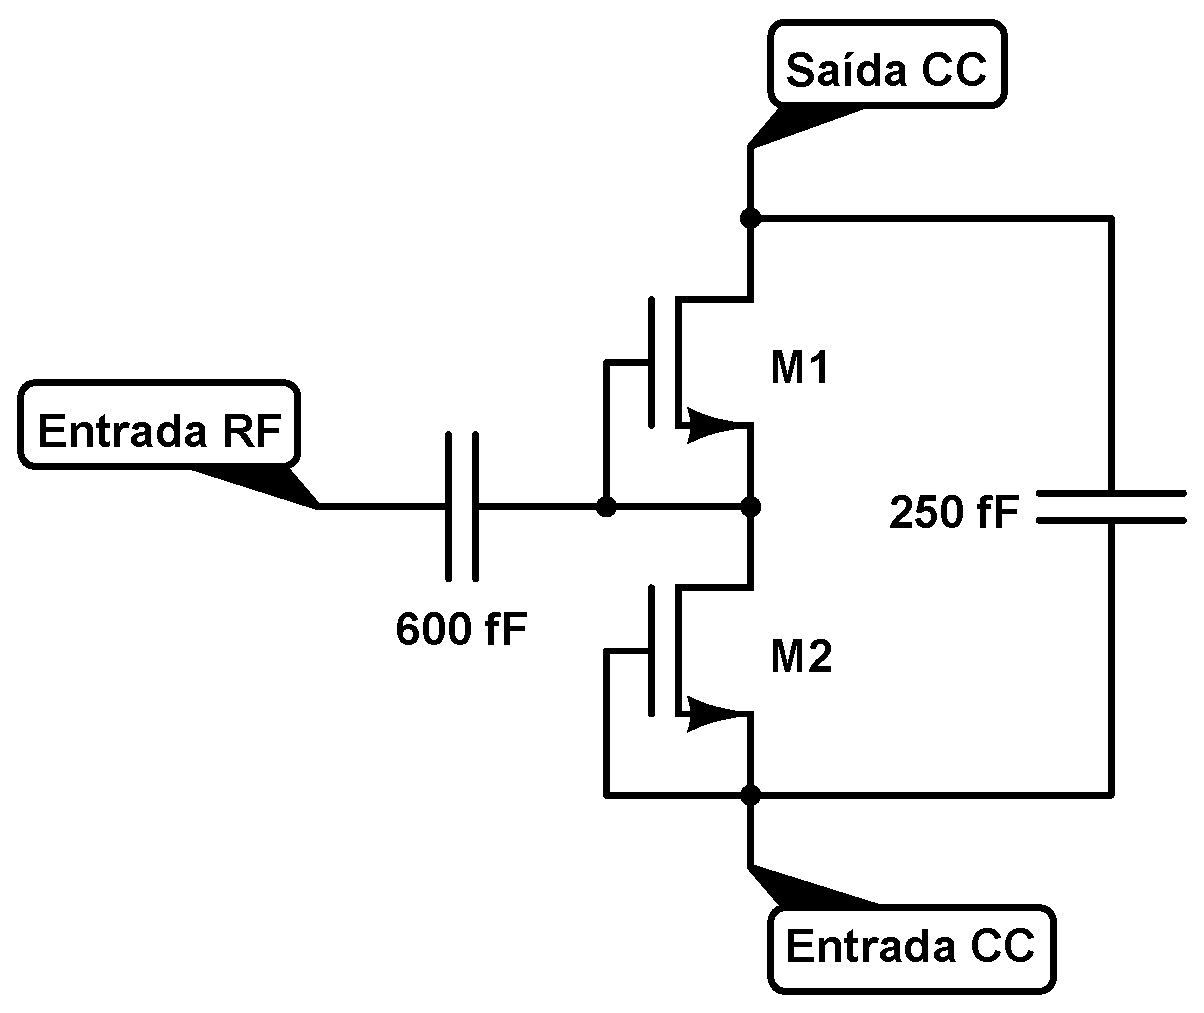
\includegraphics[width=0.5\linewidth]{rectifier-cell.eps}
	\end{center}
	\legend{Fonte: adaptação de \citeonline{YEAGER:2009}}
\end{figure}

\begin{figure}[!h]
	\caption{\label{fig:rectifier_6_cells}Esquemático do retificador implementado}
	\begin{center}
		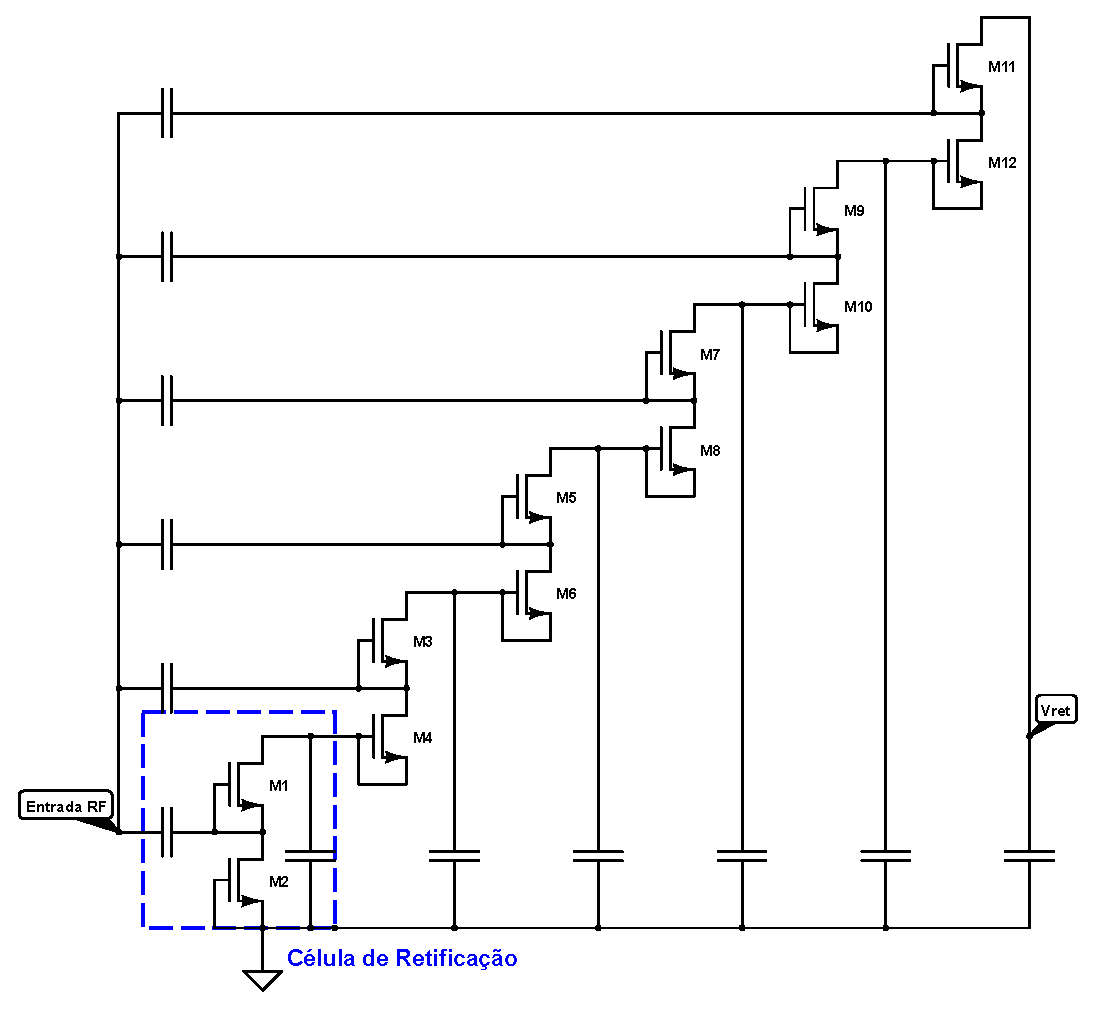
\includegraphics[width=\linewidth]{6-stages-rectifier.eps}
	\end{center}
	\legend{Fonte: autor}
\end{figure}

A célula utilizada é apresentada na Figura \ref{fig:rectifier_cell}. Nela, transistores de $V_t$ nulo são ligados como diodos e os capacitores servem como filtro cc e armazenamento temporário de carga para o estágio de retificação. O retificador foi montado com a alocação em série de seis células, como no diagrama da Figura \ref{fig:rectifier_6_cells}. Foram realizadas simulações transientes com o intuito de avaliar as características de retificação e elevação de tensão.


%\section{Modulador}
%A modulação do sinal base é importante para a viabilização da transmissão de dados entre a etiqueta e o leitor. O estudo de técnicas de modulação e suas viabilidades energéticas foge do escopo deste trabalho.

%\citeonline{KARTHAUS:2003}, \citeonline{VITA:2005} e \citeonline{KELLOGG:2014} utilizam topologias baseadas no retroespalhamento, com foco no baixo consumo energético. \citeonline{KARTHAUS:2003} utilizam modulação {PSK} com a justificativa de que alto rendimento para geração cc e alta potência na onda modulada são alcançados, simultaneamente. Apresentam justificativa matemática para as proposições realizadas. \citeonline{VITA:2005} comparam modulações {ASK} e {PSK} baseadas nessa topologia, com detalhamento matemático.

%A abordagem adotada neste trabalho foi a mesma de \citeonline{YEAGER:2009}. Como se observa na Figura \ref{fig:schematic}, um transistor, cujo porta está conectado à saída da mensagem digital, age como modulador. Quando o sinal base tiver valor lógico $1$, o transistor é polarizado, ligando a antena ao referencial comum. Quando o sinal base tiver valor lógico $0$, o transistor entra em corte. Dessa forma o sinal da antena não é influenciado pela etiqueta.

%A Figura \ref{fig:mod_ask} exemplifica este processo. As dimensões utilizadas para o modulador foram as mesmas adotadas por \citeonline{YEAGER:2009}. Nela, a informação presente no sinal base é modulada numa portadora senoide.

%\begin{figure}[!htb]
%	\caption{\label{fig:mod_ask}Modulação de um sinal quadrado com ciclo de trabalho de 50\%}
%	\begin{center}
%		\includegraphics[width=0.8\linewidth]{mod_ask.png}
%	\end{center}
%	\legend{Fonte: autor}
%\end{figure}


\section{Referencial de Tensão}
A literatura no que diz respeito a circuitos que funcionam como referencial de tensão possui elementos já consolidados e amplamente utilizados. Este módulo não é crítico para o sistema, portanto uma topologia padrão de livro foi utilizada, a fim de se conseguir os níveis de tensão de $1,2~V$ e $0,7~V$ desejados para futura regulação.

Características desejadas para este circuito eram independência do nível de tensão e da temperatura do sistema. O nível {CC} da tensão não-regulada ($V_{nr}$) não pode ser previsto com precisão, devido às incertezas de distância do leitor, tempo de exposição ao sinal da fonte, dependências da temperatura do retificador e dos demais componentes. Essa, inclusive, é outra variável que não pode ser precisamente definida. Existe, nesse contexto, a necessidade de se buscar soluções de independência dessas variáveis para a tensão de referencial.

Circuitos com esse tipo de independência são conhecidos na literatura como \textit{bandgap references} \cite{ALLEN:2002}. Topologias para o projeto de circuitos assim existem em \citeonline{MARTIN:1997} e \citeonline{ALLEN:2002}, em tecnologias CMOS, bipolar e BiCMOS. A modelagem aqui proposta é analisada por \citeonline{ALLEN:2002} e também utilizada por \citeonline{YEAGER:2009}.

O regulador implementado é apresentado na Figura \ref{fig:bandgap}. Segundo \citeonline{YEAGER:2009}, precisão na tensão de saída é garantida a partir de uma precisa relação entre as resistência utilizadas. Esta precisão pode ser alcançada a partir de um \textit{layout} intercalado entre as resistências, de modo a garantir que as nuâncias de processo sejam homogeneamente aplicadas a ambas. Os transistores de junção utilizados são diodos de junção parasítica, caracterizados na tecnologia utilizada.

\begin{figure}[!htb]
	\caption{\label{fig:bandgap}Circuito referencial de tensão implementado}
	\begin{center}
		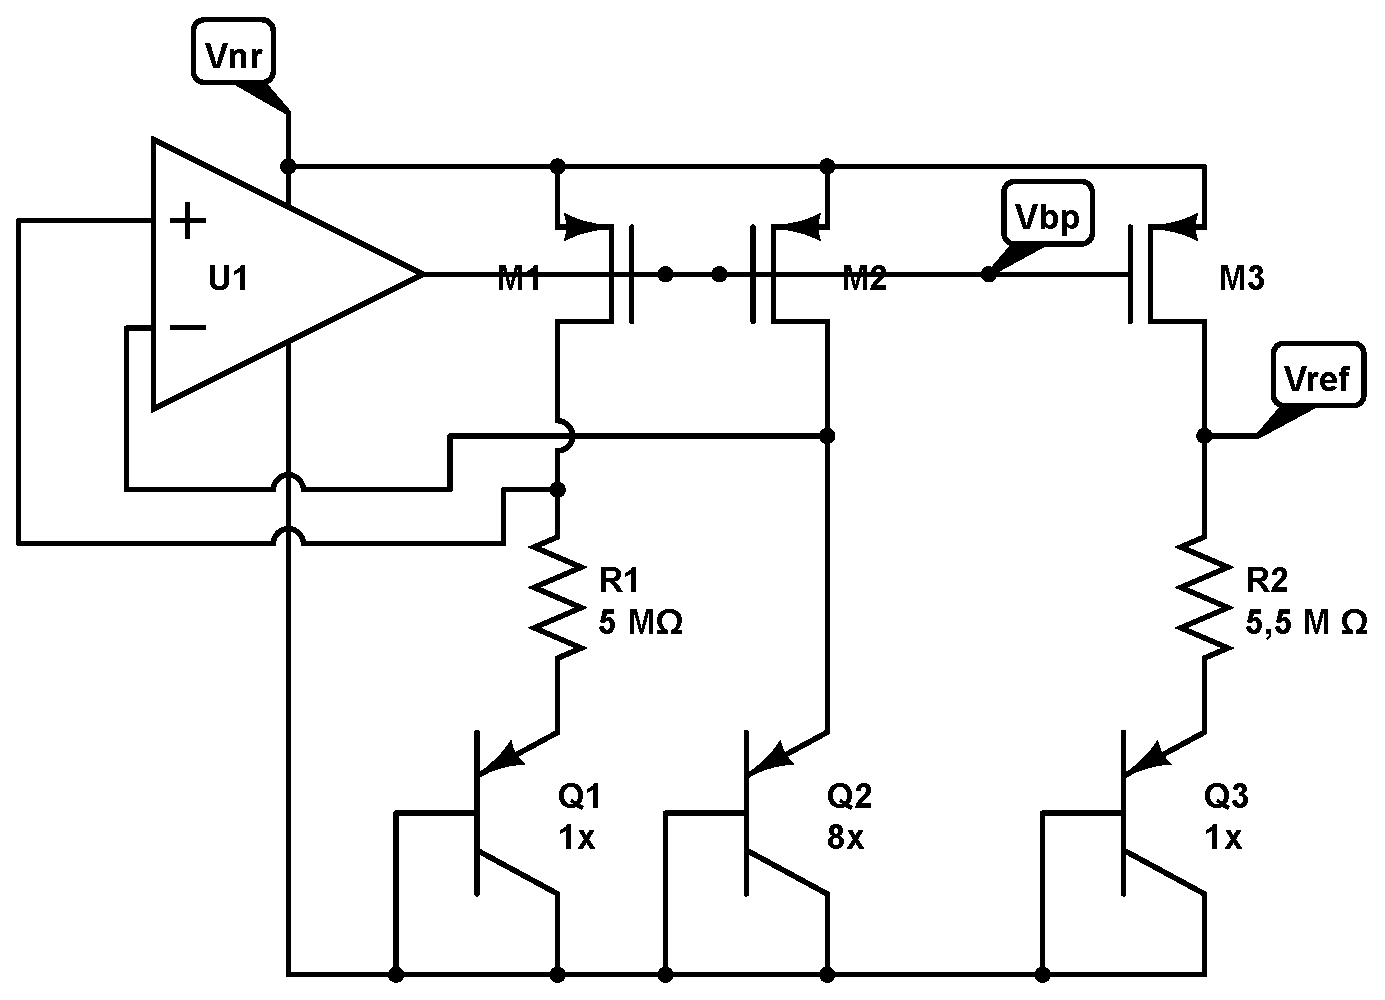
\includegraphics[width=0.8\linewidth]{bandgap-reference.eps}
	\end{center}
	\legend{Fonte: adaptado de \citeonline{YEAGER:2009}}
\end{figure}

No retificador em questão, as resistências {R1} e {R2} têm a função de ajustar as curvas de variação da tensão em seus ramos com a temperatura, de modo que a diferença resultante do amplificador {U1} seja independente dessa variável.

\section{Referencial de Corrente}
Para o desenvolvimento do sistema proposto, viu-se a necessidade de se gerar valores de corrente precisos para a polarização de transistores. Devido à imprecisão da fonte de tensão não-regulada, é importante que as correntes de referência sejam independentes da alimentação o máximo possível.

O circuito implementado para gerar os referenciais de $50~nA$ utilizados na polarização de fontes de corrente foi projetado a partir de um modelo apresentado por \citeonline{MARTIN:1997}, como apresentado na \autoref{fig:bias_current}.

\begin{figure}[!h]
	\caption{\label{fig:bias_current}Circuito referencial de corrente implementado}
	\begin{center}
		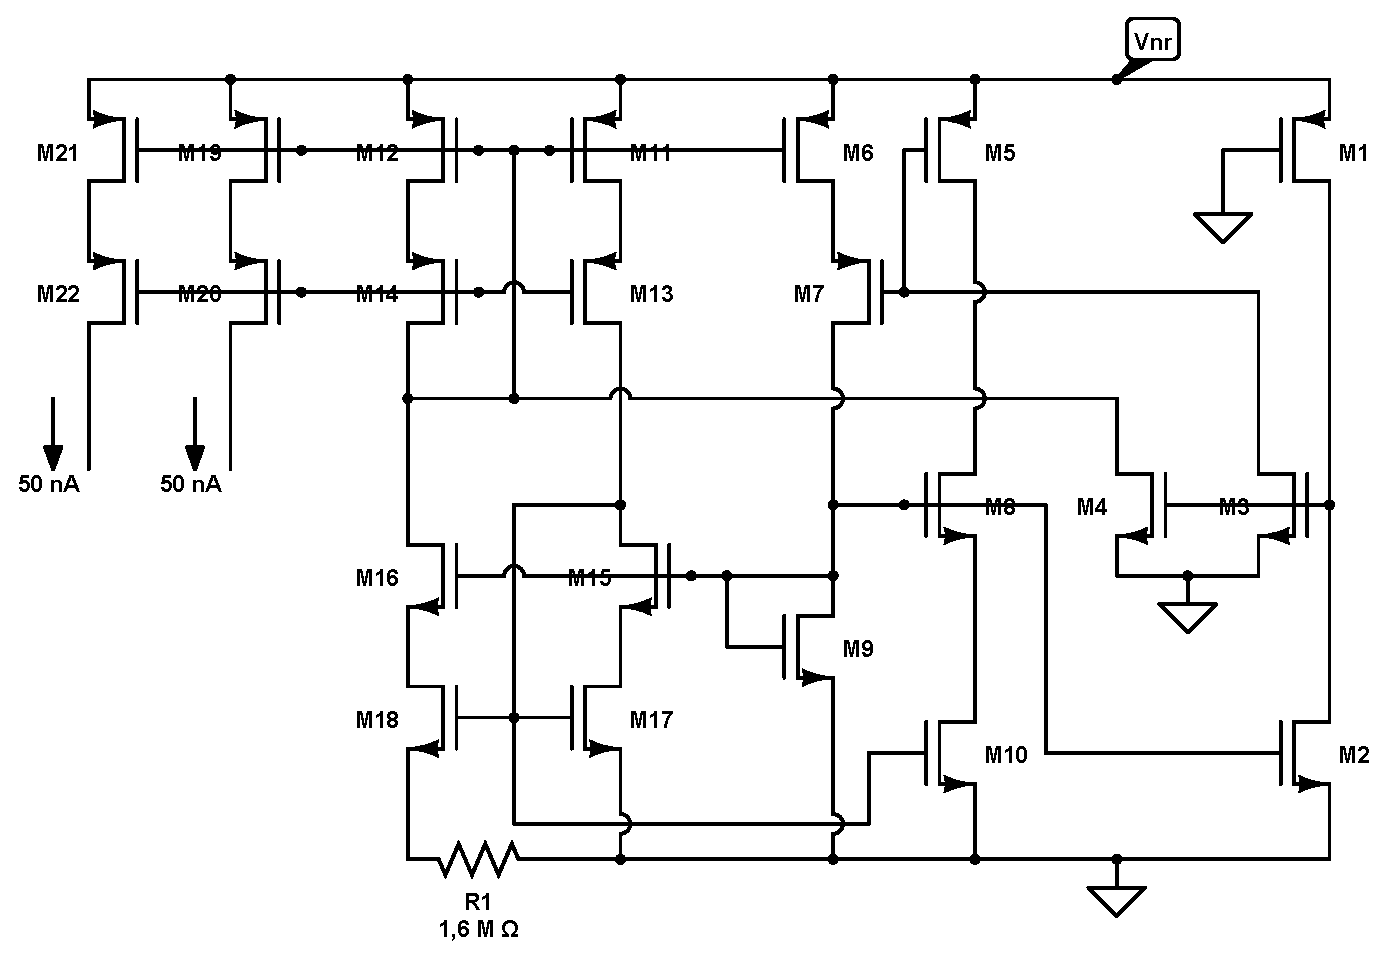
\includegraphics[width=\linewidth]{bias-current.eps}
	\end{center}
	\legend{Fonte: adaptado de \citeonline{MARTIN:1997}}
\end{figure}

Os pares de transistores {M19} e {M20}, bem como {M21} e {M22}, representam as fontes de corrente do sistema. Na ordem, da esquerda à direita, estão os circuitos de espelho de corrente, polarização e inicialização. São utilizadas configurações de fonte de corrente devido aos baixos valores de corrente desejados. Segundo \citeonline{YEAGER:2009}, os valores transientes levam um bom tempo para se estabilizarem, vulnerabilizando as tensões de referência. Outro fator que favorece o uso de fontes {PMOS} é o fato de circuitos chaveados, como moduladores, poderem injetar ruídos nas tensões de referência dos transistores {NMOS}.

\begin{citacao}
	É possível incorporar espelhos de corrente de alta largura em circuitos de polarização de transcondutância constante [...]. Essa modificação minimiza bastante a maioria das imperfeições de segunda ordem causadas pela impedância de saída finita dos transistores, sem restringir muito a oscilação de sinais. \cite{MARTIN:1997}.
\end{citacao}

As fontes de corrente utilizam uma configuração em cascata para aumento da impedância de saída, garantindo maior estabilidade à corrente. Foram utilizados transistores de camada de óxido espessa neste módulo. Uma configuração similar foi utilizada por \citeonline{YEAGER:2009}.

\begin{citacao}
	Apesar do uso de dispositivos de camada de óxido espessa, o \textit{bias generator} inicia confiavelmente com $0,6~V$. A alta impedância de saída de dispositivos em cascata, mesmo em operação sub-limiar, mantém uma corrente de saída notavelmente constante de $0,6~V$ a $3,6~V$. \cite{YEAGER:2009}.
\end{citacao}


\section{Regulador de Tensão}
A função do regulador de tensão é a de prover uma fonte de valor específico de onde se possa drenar a energia necessária para o funcionamento de dispositivos. Neste trabalho, propõe-se um circuito regulador para a criação de dois níveis distintos de tensão. Seguiu-se a topologia apresentada por \citeonline{YEAGER:2009}.

As fontes criadas são de $1,2~V$ para circuitos analógicos e a de $0,7~V$ para digitais. É possível se obter valores distintos de tensão regulada a partir da mudança do valor de referência, devido à realimentação do módulo.

\begin{figure}[!h]
	\caption{\label{fig:regulator}Circuito regulador de tensão implementado}
	\begin{center}
		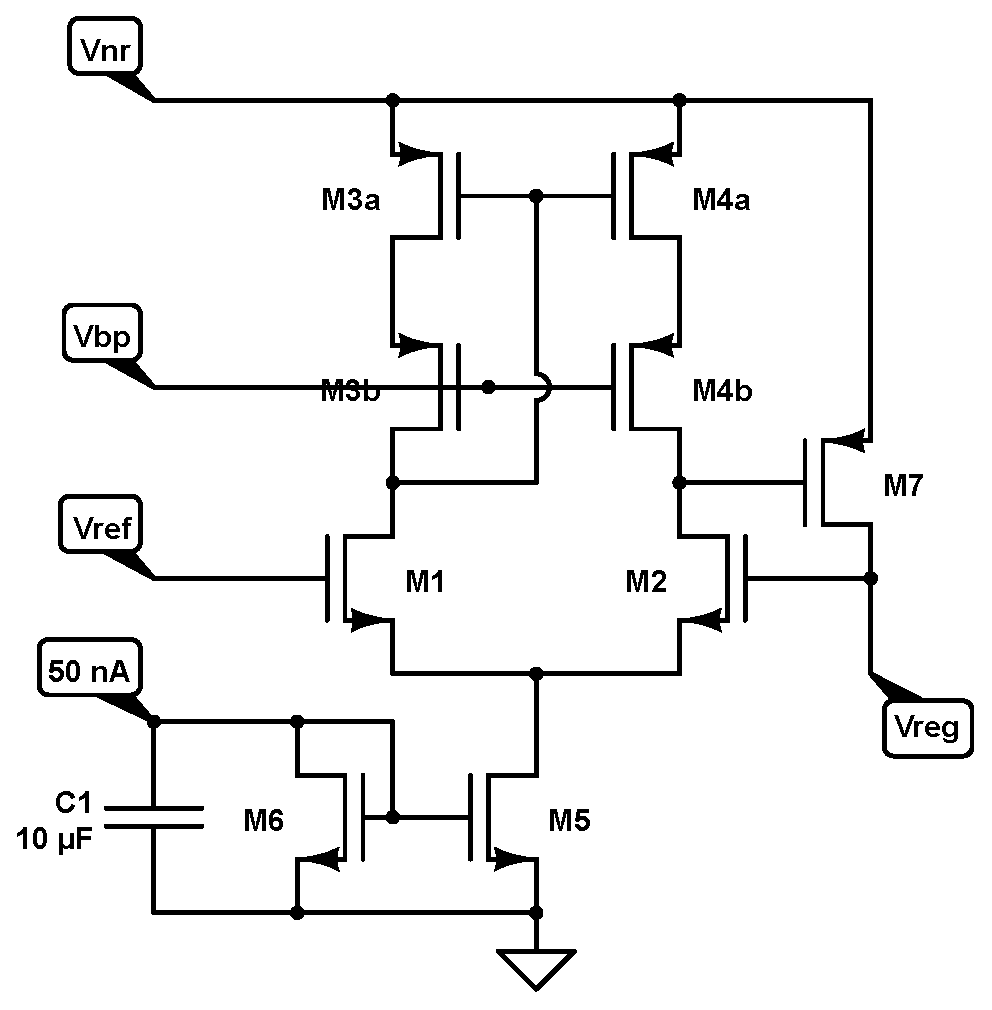
\includegraphics[width=0.8\linewidth]{voltage-regulator.eps}
	\end{center}
	\legend{Fonte: adaptado de \citeonline{YEAGER:2009}}
\end{figure}

O circuito implementado é apresentado na Figura \ref{fig:regulator}. O regulador é proposto a partir de um comparador. A entrada não-inversora do amplificador é ligada ao valor de referência gerada pelo circuito referencial de tensão, $V_{ref}$, e a inversora é realimentada da saída, servindo como base para a estabilização do circuito. A utilização do esquema em cascata no comparador aumenta o ganho da estrutura, que é baixo devido à operação em região sub-limiar. A tensão $V_{bp}$, utilizada para polarizar os transistores da cascata, é proveniente dos circuitos referenciais de tensão. A polarização do comparador é feita com a utilização da saída do circuito referencial de corrente. O transistor {M6} gera o nível de polarização para {M5}, funcionando como um espelho de corrente. O transistor {M7}, chamado por \citeonline{YEAGER:2009} de transistor de passagem, deve possuir largura o suficiente para permitir que a corrente destinada à carga seja transmitida sem que haja muita dissipação de energia.


\section{Síntese}
Neste capítulo são abordadas as características de projeto dos módulos principais que compõem um \textit{front-end} analógico. O \autoref{Resultados} segue com os resultados observados nas simulações de cada um dos módulos implementados e, em seguida, da união deles em um sistema completo. Discussões acerca desses resultados são feitas, bem como análises pertinentes a respeito dos consumos energéticos e rendimentos obtidos.


%\section{Demodulador}
% TODO - Buscar RFID authentication protocol for low-cost tags - Informação sobre os tipos de protocolos usados
%O demodulador é o módulo responsável por recuperar a informação presente no sinal recebido do leitor. Este módulo é bastante dependente da aplicação onde é utilizado.

% TODO - Artigos em Pulse-Interval Encoding
%Para este trabalho, tomou-se como base o protocolo Gen2. Nele, a comunicação da etiqueta emprega codificação por intervalo de pulso. Especificamente, a duração da largura do pulso positivo determina se cada bit é zero ou um \cite{YEAGER:2009}. O demodulador aqui apresentado segue a mesma topologia adotada por \citeonline{YEAGER:2009}.

%\begin{citacao}
%	É, essencialmente, um amplificador operacional de 2 estágios; o primeiro estágio provê conversão diferencial com ganho, pelo menos, unitário na largura de banda do sinal. O segundo estágio significativamente aumenta a amplitude do sinal para atingir uma variação no nível lógico. \cite{YEAGER:2009}.
%\end{citacao}

%\begin{figure}[!bh]
%	\caption{\label{fig:demodulator}Circuito demodulador implementado}
%	\begin{center}
%		\includegraphics[width=0.9\linewidth]{demodulator.png}
%	\end{center}
%	\legend{Fonte: adaptado de \citeonline{YEAGER:2009}}
%\end{figure}

%O circuito implementado é apresentado na Figura \ref{fig:demodulator}. O sinal base, demodulado pelo amplificador operacional, é remetido à tensão digital para, finalmente, ser transmitido ao núcleo digital da etiqueta. Essa mudança se dá através de dois amplificadores inversores em série.

%Não é o foco deste trabalho definir o protocolo utilizado. O demodulador empregado é apresentado a título de exemplo e como forma de apresentar um \textit{front-end} completo.

%Topologias de demoduladores para diferentes tipos de modulação são analisadas por estudos em aplicações {RFID}. \citeonline{NAKAMOTO:2006} compara a demodulação {ASK} (modulação por deslocamento de amplitude, em português) tradicional com um método de sensibilidade de corrente apresentado. \citeonline{KARTHAUS:2003} apresenta uma solução para demodulação de sinais modulados com modulação {PWM} (modulação por largura de pulso, em português). As vantagens e desvantagens de cada uma variam com a aplicação.

